\documentclass[Main.tex]{subfiles}
 
\begin{document}

\begin{addmargin}[18em]{0em} 74 \ \ \ \ КНИГА I ПРЕДЛ. XLVIII. ТЕОРЕМА \end{addmargin}

\begin{multicols}{2}
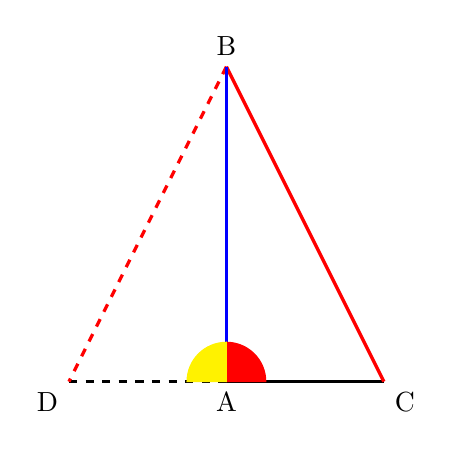
\begin{tikzpicture}
    \draw[very thick,dashed] (0,0) -- (2,0) node[anchor=north] {A};
    \draw[very thick] (2,0) -- (4,0) node[anchor=north west] {C};
    \draw[red, very thick] (4,0) -- (2,4) node[anchor=south, black] {B};
    \draw[dashed,red,very thick] (2,4) -- (0,0) node[anchor=north east, black] {D};
    \draw[blue,very thick] (2,0) -- (2,4);
    \begin{scope}[xshift=2cm]
        \filldraw[fill=red,color=red] 
            (0:0.5cm)
            -- (0,0)
            -- (90:0.5cm)
            arc[start angle=90, end angle=0, radius=0.5cm]
            -- cycle;
        \filldraw[fill=yellow,color=yellow] 
            (180:0.5cm)
            -- (0,0)
            -- (90:0.5cm)
            arc[start angle=90, end angle=180, radius=0.5cm]
            -- cycle;
    \end{scope}
\end{tikzpicture}

\vfill\null
\columnbreak

\lettrine[findent=2pt]{\fbox{\textbf{Е}}}{ }\textit{сли в треугольнике квадрат одной стороны 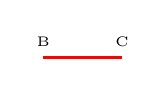
\begin{tikzpicture}
    \draw[red, very thick] node[font = {\tiny},black,above] {B} (0,0) -- (1,0) node[font = {\tiny},black,above] {C};
\end{tikzpicture} равен сумме квадратов двух других сторон 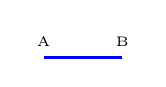
\begin{tikzpicture}
    \draw[blue, very thick] node[font = {\tiny},black, above] {A} (0,0) -- (1,0) node[font = {\tiny},black, above] {B};
\end{tikzpicture} и 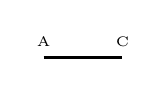
\begin{tikzpicture}
    \draw[very thick] node[font = {\tiny},above] {A} (0,0) -- (1,0) node[font = {\tiny},above] {C};
\end{tikzpicture}, то угол 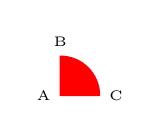
\begin{tikzpicture}
    \filldraw[fill=red,color=red]
            (0:0.5cm) node[font = {\tiny}, black, right] {C}
            -- (0,0) node [font = {\tiny},black, left] {A}
            -- (90:0.5cm) node [font = {\tiny},black, above] {B}
            arc[start angle=90, end angle=0, radius=0.5cm]
            -- cycle;
\end{tikzpicture}, заключенный между этими двумя сторонами прямой.
}

\begin{center}
    Проведем \begin{tikzpicture}
    \draw[dashed, very thick] node[font = {\tiny},black,above] {A} (0,0) -- (1,0) node[font = {\tiny},black,above] {D};
\end{tikzpicture} $\perp$ 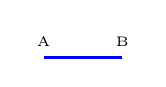
\begin{tikzpicture}
    \draw[blue, very thick] node[font = {\tiny},black,above] {A} (0,0) -- (1,0) node[font = {\tiny},black,above] {B};
\end{tikzpicture}

и = \begin{tikzpicture}
    \draw[very thick] node[font = {\tiny},black,above] {A} (0,0) -- (1,0) node[font = {\tiny},black,above] {С};
\end{tikzpicture} (пр. $I._{II}, I._3$)

также проведем \begin{tikzpicture}
    \draw[red, dashed, very thick] node[font = {\tiny},black,above] {B} (0,0) -- (1,0) node[font = {\tiny},black,above] {D};
\end{tikzpicture}.

Поскольку \begin{tikzpicture}
    \draw[dashed, very thick] node[font = {\tiny},black,above] {A} (0,0) -- (1,0) node[font = {\tiny},black,above] {D};
\end{tikzpicture} = \begin{tikzpicture}
    \draw[very thick] node[font = {\tiny},black,above] {A} (0,0) -- (1,0) node[font = {\tiny},black,above] {С};
\end{tikzpicture} (постр.)

\begin{tikzpicture}
    \draw[dashed, very thick] node[font = {\tiny},black,above] {A} (0,0) -- (1,0) node[font = {\tiny},black,above] {D};
\end{tikzpicture}$\ ^2$ = \begin{tikzpicture}
    \draw[very thick] node[font = {\tiny},black,above] {A} (0,0) -- (1,0) node[font = {\tiny},black,above] {С};
\end{tikzpicture}$ ^2$;

$\implies$ \begin{tikzpicture}
    \draw[dashed, very thick] node[font = {\tiny},black,above] {A} (0,0) -- (1,0) node[font = {\tiny},black,above] {D};
\end{tikzpicture}$\ ^2$ + 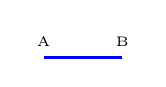
\begin{tikzpicture}
    \draw[blue, very thick] node[font = {\tiny},black,above] {A} (0,0) -- (1,0) node[font = {\tiny},black,above] {B};
\end{tikzpicture}$\ ^2$ = \begin{tikzpicture}
    \draw[very thick] node[font = {\tiny},black,above] {A} (0,0) -- (1,0) node[font = {\tiny},black,above] {С};
\end{tikzpicture}$ ^2$ + 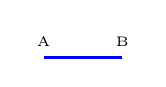
\begin{tikzpicture}
    \draw[blue, very thick] node[font = {\tiny},black,above] {A} (0,0) -- (1,0) node[font = {\tiny},black,above] {B};
\end{tikzpicture}$\ ^2$

но \begin{tikzpicture}
    \draw[dashed, very thick] node[font = {\tiny},black,above] {A} (0,0) -- (1,0) node[font = {\tiny},black,above] {D};
\end{tikzpicture}$\ ^2$ + 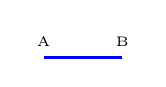
\begin{tikzpicture}
    \draw[blue, very thick] node[font = {\tiny},black,above] {A} (0,0) -- (1,0) node[font = {\tiny},black,above] {B};
\end{tikzpicture}$\ ^2$ = \begin{tikzpicture}
    \draw[red, dashed, very thick] node[font = {\tiny},black,above] {B} (0,0) -- (1,0) node[font = {\tiny},black,above] {D};
\end{tikzpicture}$\ ^2$ (пр. $I._{47}$),

и \begin{tikzpicture}
    \draw[very thick] node[font = {\tiny},black,above] {A} (0,0) -- (1,0) node[font = {\tiny},black,above] {С};
\end{tikzpicture}$ ^2$ + 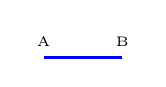
\begin{tikzpicture}
    \draw[blue, very thick] node[font = {\tiny},black,above] {A} (0,0) -- (1,0) node[font = {\tiny},black,above] {B};
\end{tikzpicture}$\ ^2$ = 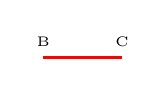
\begin{tikzpicture}
    \draw[red, very thick] node[font = {\tiny},black,above] {B} (0,0) -- (1,0) node[font = {\tiny},black,above] {C};
\end{tikzpicture}$\ ^2$ (гип.)

$\implies$ \begin{tikzpicture}
    \draw[red, dashed, very thick] node[font = {\tiny},black,above] {B} (0,0) -- (1,0) node[font = {\tiny},black,above] {D};
\end{tikzpicture}$\ ^2$ = 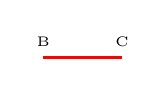
\begin{tikzpicture}
    \draw[red, very thick] node[font = {\tiny},black,above] {B} (0,0) -- (1,0) node[font = {\tiny},black,above] {C};
\end{tikzpicture}$\ ^2$,

$\implies$ \begin{tikzpicture}
    \draw[red, dashed, very thick] node[font = {\tiny},black,above] {B} (0,0) -- (1,0) node[font = {\tiny},black,above] {D};
\end{tikzpicture} = 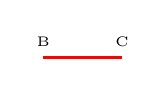
\begin{tikzpicture}
    \draw[red, very thick] node[font = {\tiny},black,above] {B} (0,0) -- (1,0) node[font = {\tiny},black,above] {C};
\end{tikzpicture};

и $\implies$ 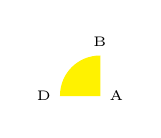
\begin{tikzpicture}
    \filldraw[fill=yellow,color=yellow] 
            (180:0.5cm) node[font = {\tiny}, black, left] {D}
            -- (0,0) node[font = {\tiny}, black, right] {A}
            -- (90:0.5cm) node[font = {\tiny}, black, above] {B}
            arc[start angle=90, end angle=180, radius=0.5cm]
            -- cycle;
\end{tikzpicture} = 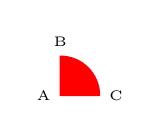
\begin{tikzpicture}
    \filldraw[fill=red,color=red]
            (0:0.5cm) node[font = {\tiny}, black, right] {C}
            -- (0,0) node [font = {\tiny},black, left] {A}
            -- (90:0.5cm) node [font = {\tiny},black, above] {B}
            arc[start angle=90, end angle=0, radius=0.5cm]
            -- cycle;
\end{tikzpicture} (пр. $I.8$),

следовательно 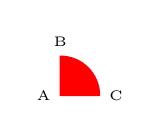
\begin{tikzpicture}
    \filldraw[fill=red,color=red]
            (0:0.5cm) node[font = {\tiny}, black, right] {C}
            -- (0,0) node [font = {\tiny},black, left] {A}
            -- (90:0.5cm) node [font = {\tiny},black, above] {B}
            arc[start angle=90, end angle=0, radius=0.5cm]
            -- cycle;
\end{tikzpicture} прямой угол.

\end{center}

\begin{flushright}
    ч. т. д.
\end{flushright}

\end{multicols}

\end{document}